\chapter{LHC-ATLAS実験}
\label{chap_TGC}

% この章では、自分の研究に関連する分野の歴史や現状について説明したり、研究を展開する上で重要となる知識の解説を行います。ここで使用している見出し「ガンマ線天文学…」はあくまで例ですが、もしCherekov Telescope Array(CTA)計画\footnote{省略語は必ず正式名称を先に書き、省略系は丸括弧に入れます。省略語はあくまで「以降このように略す」という用途だからです。また、日本語文章中で使う丸括弧は()ではなく()です。}に携わる院生の書く修士論文であれば、ガンマ線天文学や宇宙線物理学全般について、現行望遠鏡とガンマ線観測の原理について、またCTA計画についての記述がこの章では期待されます。

% 場合によっては「序論」と合体させても良いですが、本章は比較的長くなり結論に直結しない情報もたくさん出てくるため、独立した章である方が読者は読みやすいでしょう。

% またこの章が長くなるときには、例えば「ガンマ線天文学」と「CTA計画」のように、2つの章に分割するというのも良いと思います。\footnote{注意書きの練習です。}


\section{ATLAS検出器}
\label{sec_ATLAS}

\subsection{ATLAS実験における座標系と変数}
図\ref{ATLAScordination}にATLAS実験で使われる2種類の座標系を示す。直交座標系は、原点を検出器中心、x軸方向をLHCの中心方向、y軸を地上方向、z軸をビーム軸方向に定義した右手系で定義する。$z>0$ の領域をA side、$z<0$の領域をC sideと呼ぶ。円筒座標系は、ビーム軸を中心とした方位角方向を$\phi$、ビーム軸からの天頂角方向を$\theta$、同型方向を$R$と定義する。$\theta$ 方向を表す変数として擬ラピデティ(Pseudorapidity)$\eta$
\begin{equation}
    \eta = -\ln(\mathrm{tan}\frac{\theta}{2})
\end{equation}
をよく利用する。2粒子の擬ラピデティの差はz軸方向のブーストに対してローレンツ不変であり、物理現象を記述する上で有用だからである。また$\eta$は検出器が覆う領域を説明する際にも利用される。本研究で扱うミューオンシステムでは、|$\eta$| < 1.05の円筒側面領域をバレル領域(barrel)、|$\eta$| > 1.05の円筒底面領域をエンドキャップ(endcap)と呼ぶ。またATLAS実験では粒子の状態を表す物理量としてz軸垂直方向の運動量(横方向運動量,\pt)やエネルギー(横方向エネルギー,$E_{\mathrm{T}}$)を利用する。陽子陽子衝突実験で実行的に衝突するクォークやグルーオンのz軸方向の運動量は不定であるのに対し、ビーム軸に垂直な方向に関しては運動量の和が0であることが保証され、不定性なく再構成できるためである。
\begin{figure} 
\centering
\includegraphics[width=16cm]{fig/Intro/ATLAScordination.pdf}
\caption[ATLAS検出器における座標系]{ATLAS検出器で用いられる座標系。ビーム軸方向をz軸、LHC中心方向をx軸正の向きとした右手系で定義される。$z>0$をA side、$z<0$をC sideと呼ぶ。円筒座標系も利用され、特に検出器を覆う領域を説明するのに$\eta$が利用される。}
\label{ATLAScordination}
\end{figure}


\subsection{ATLAS検出器における超伝導磁石}
ATLAS検出器では荷電粒子の運動量を測定するため2種類の超伝導磁石が設置されている。図\ref{ATLASmagnet}に各磁石の配置図を示す。ソレノイド磁石は内部飛跡検出器とカロリメーターの間の領域に設置され、内部飛跡検出器内で荷電粒子を曲げる役割をもつ。トロイド磁石はカロリメーターの外側に設置され、内部検出器を透過してきたミューオンを曲げるのに利用される。バレル部とエンドキャップ部のトロイド磁石はお互いの干渉を避けるため22.5度ずらして設置されるが、双方の磁場が影響を与えた結果、eta方向にも$\phi$方向にも均一ではない。そのためミューオンの運動量は飛跡の曲率から直接逆算することが難しく、直線飛跡との角度比較を元に行われる。その方法の詳細は\ref{}説で説明する。

\begin{figure} 
    \centering
    \includegraphics[width=16cm]{fig/Intro/ATLASmagnet.pdf}
    \caption[超伝導磁石の配置]{超伝導磁石の配置\cite{JINST:2008}。内部飛跡検出器を囲うようにソレノイド磁石が、カロリメーターの外側にトロイド磁石が設置されている。トロイド磁石はバレル部とエンドキャップ部で干渉の内容22.5度ずらして設置される。}
    \label{ATLASmagnet}
\end{figure}


\subsection{ミューオンスペクトロメーター}
ミューオンスペクトロメーターはATLAS検出器最外層に設置された検出器で、カロリーメーターを透過したミューオンの横方向運動量を測定する役割を担う。ミューオンスペクトロメーターは主にMonitored Drift Tube(MDT)、Resistive Plate Chamber(RPC)、Thin Gap Chamber(TGC)検出器で構成される。RPCとTGCは時間分解能に優れ、応答時間も高速であるためトリガーに利用される。MDTは位置分解能に優れているため、運動量の精密測定に利用される。トロイド磁場内部にはトリガー用の検出器としてTile Calorimeter、TGC EI、RPC BIS78、NSW、が設置されている。

各検出器の設置される領域を図\ref{Muonspectrometer2}に示す。ミューオンスペクトロメーターはトロイドマグネットの磁場構造に合わせて8回対称になっており、マグネットや支持構造と干渉しないよう、$\phi$方向にLarge sector、Small sectorという2種類のsectorに分かれている。トリガー用の検出器として|$eta$| < 1.05のバレル領域ではRPC、1.05 < |$\eta$| < 2.4のエンドキャップ領域ではTGCが最外層に設置される。エンドキャップ領域において磁場内部の検出器カバーする$\eta$、$\phi$領域を図\ref{}に示す。1.3 < $eta$ < 2.4の領域はNSWが網羅的にカバーしており、1.05 < $eta$ < 1.3領域ではTGC EI、RPC BIS78、Tile カロリメーターがそれぞれ補的にカバーする。

\begin{figure} 
\centering
\includegraphics[width=16cm]{fig/Intro/Muonspectrometer.pdf}
\caption[高輝度LHC-ATLAS実験でのミューオンスペクトロメーターの断面図]{高輝度LHC-ATLAS実験でのミューオンスペクトロメーターの断面図.\cite{tdr_phase2muon_2017017}
}
\label{Muonspectrometer2}
\end{figure}


%TGC検出器
Thin Gap Chamber(TGC)は1.05 < |$\eta$| < 2.4のエンドキャップ領域をカバーする円盤型のミューオントリガー検出器である。TGCはEndcapトロイドマグネットより内側に位置するEndcap Innner(EI)と外側に位置するBig Wheel(BW)に大別される。図\ref{TGC_picture}にBWの写真を示す。TGC BWはz方向に3つのステーションが連なって構成され、衝突点に近い方からM1、M2、M3ステーションと呼ぶ。各ステーションは2層または3層のガス層で構成されており、2層のものをdoublet、3層のものをtripletと呼ぶ。BWではM1がtriplet、M2、M3がdoubletである。

\begin{figure} 
\centering
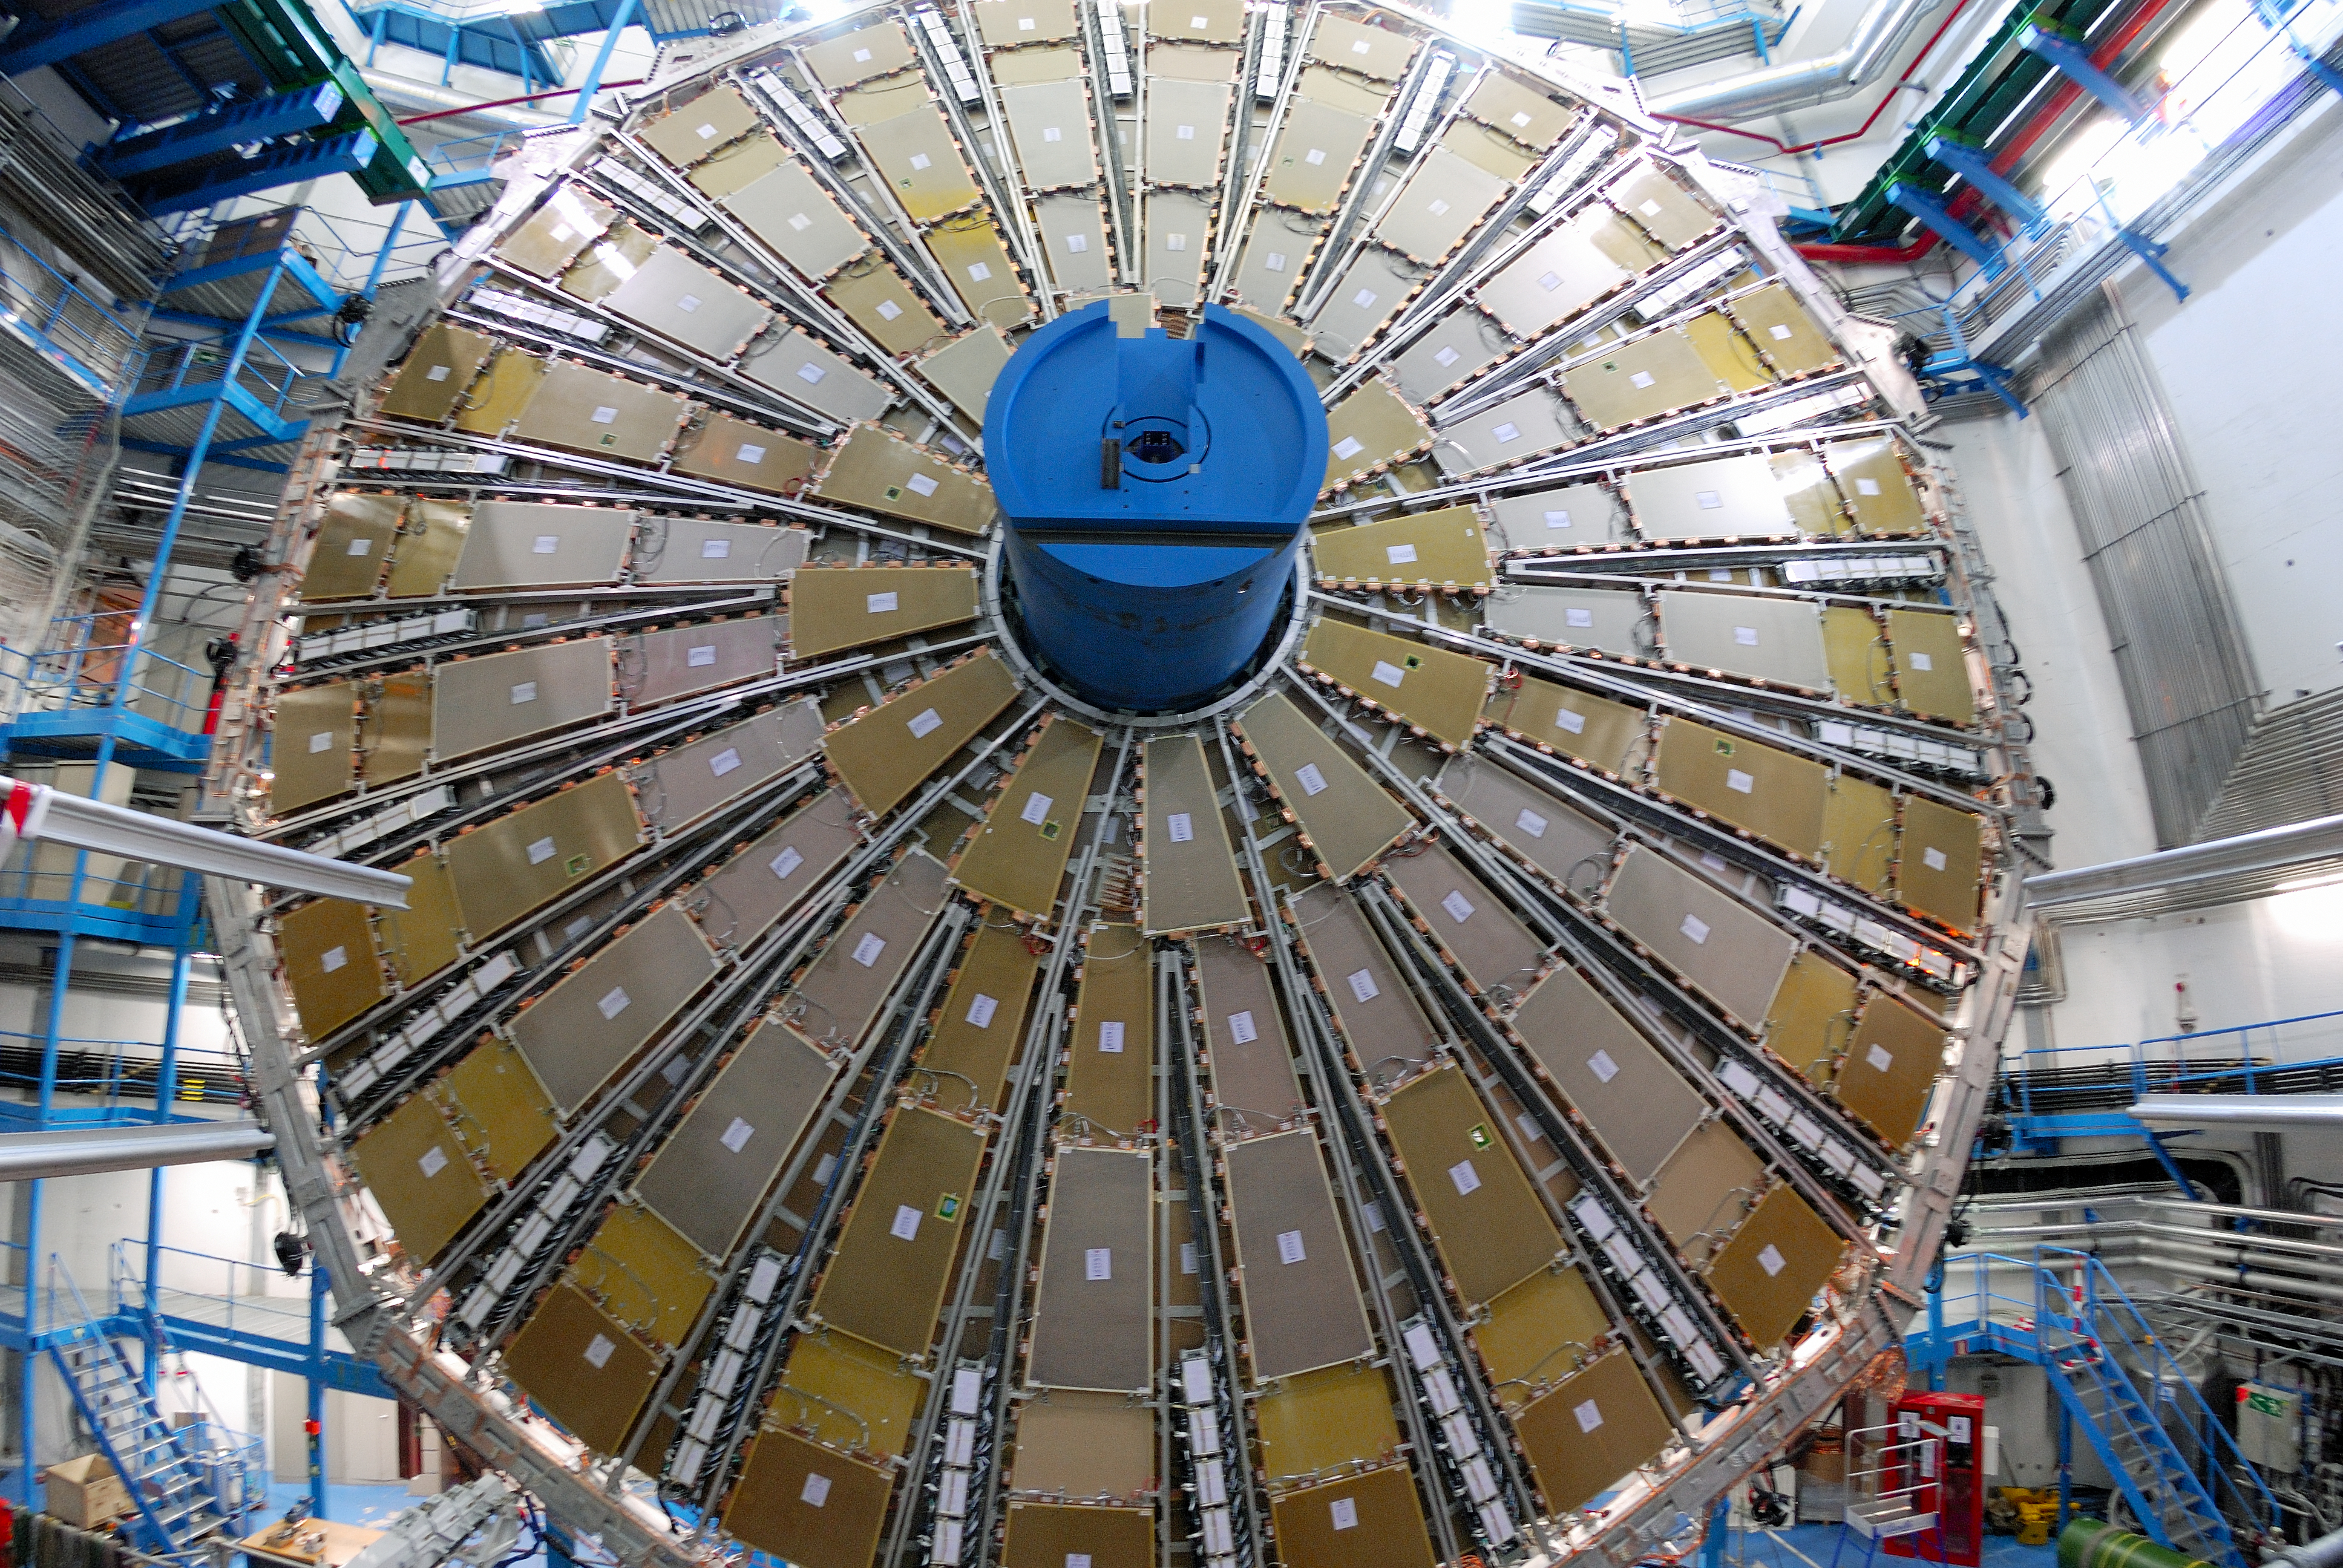
\includegraphics[width=16cm]{fig/Intro/TGC_picture.jpg}
\caption[TGC検出器]{TGC検出器の正面写真(M1)\cite{cern_document_server}}
\label{TGC_picture}
\end{figure}

TGCチェンバーの構造を図\ref{TGC_structure}に示す。TGCはアノードワイヤー間隔が1.8mm、アノードとカソードストリップの間隔が1.4 mmであるMWPCである。ワイヤーはR方向、ストリップは$\phi$方向に直交して張られており、2次元位置を読み出しが可能である。ガス層には$CO_2/n-C_5H_{12}$が55:45で混合されたガスが充填されている。

\begin{figure}
\begin{minipage}[b]{.5\linewidth}
\centering
\includegraphics[height=5cm]{fig/Intro/TGC_structure.pdf}
\subcaption{TGCチェンバーの断面図}
\end{minipage}%
\begin{minipage}[b]{.5\linewidth}
\centering
\includegraphics[height=5cm]{fig/Intro/TGC_crosssection.pdf}
\subcaption{TGC doubletとtripletの断面図}
\end{minipage}%
\caption[TGCチェンバーの断面図]{(a)はTGCチェンバーの断面図を表す\cite{JINST:2008}。ワイヤーとストリップが直交して張られていることがわかる。(b)はTGC doubletとtripletの断面図である。それぞれ2層、3層のガスギャップで構成されており、各ガスギャップの間はペーパーハニカムにより満たされている。}
\label{TGC_structure}
\end{figure}


荷電粒子がTGCに入射すると、荷電粒子によりガス分子が電離される。電離した電子はワイヤーに印加された2.8 kVの電圧によりワイヤー方向に集められ、ワイヤー付近に到達すると強い電場により電子雪崩を生じる。ワイヤーでは電子雪崩で生じた正イオンのドリフトが、ストリップではそれらの鏡像電荷が電流信号として検出される。

TGC検出器はトリガー用の検出器であり、ガスギャップが薄く、ワイヤー間隔が小さいため時間応答がよい。これにより陽子衝突頻度である25nsより細かな時間分解能でミューオンを検出し、そのミューオンがどの陽子バンチ衝突に由来するのかを識別(Bunch Crossing IDentification, BCID)することができる。一方、TGC検出器はそれほど高い位置分解能が求められていないため、ワイヤー電極を4 ~ 20本まとめてから読み出しを行う。結果としてワイヤー、ストリップは合計32万チャンネルをもつ。


\section{ATLAS実験におけるTDAQシステム}
\label{sec_TDAQ}

\subsection{Run3でのTDAQシステム}
\label{subsec_run3TDAQ}
\ref{chap_Intro}節で述べたようにLHCでは25 nsの間隔で陽子バンチが衝突するため、衝突で生じたすべてのデータを保存することはできない。限られた読み出し帯域とオフラインの計算リソースを最大限有効活用するためには興味のある衝突事象のみを記録するトリガーが重要となる。またトリガー判定がなされたイベントに対して正しくデータを取得するには、トリガーシステムとデータ取得(data acquisition,DAQ)システムが連動して機能する必要がある。ATLAS実験では、トリガーとデータ取得をまとめてTrigger and Data Acquisition(TDAQ)システムと呼ぶ。図\ref{Run3_TDAQ}にRun3におけるTDAQシステムの概要を示す。ATLASのトリガーシステムはLevel-1という初段のハードウェアトリガーと、それに続くHigh Level Trigger(HLT)という後段のソフトウェアトリガーから構成される。

\begin{figure} 
\centering
\includegraphics[width=16cm]{fig/Intro/Run3_TDAQ.pdf}
\caption[Run3におけるTDAQシステムの概要]{Run3におけるTDAQシステムの概要\cite{Run3_TDAQ}。トリガーシステムはLevel-1 Triggerという初段ハードウェアトリガーとHigh Level Trigger(HLT)という後段のソフトウェアトリガーから構成される。L1 TriggerはL1 CaloとL1 Muonに大別されCTPで総合的なトリガー判定がなされる。L1 TriggerをパスしたイベントはHLTでより精度の高いトリガー判定が行われ、CERN Permanent Strageに保存される。 }
\label{Run3_TDAQ}
\end{figure}

\subsubsection{Level-1 Trigger}
\vskip0.5\baselineskip
Level-1 Triggerは25 ns間隔で行われるすべての陽子バンチ衝突事象の中から、物理的に興味のあるオブジェクトを含むイベントを大まかに選別する初段トリガーである。L1 Triggerによってイベントレートは40 MHzから100 kHzまで削減される。L1 Triggerは大量のデータを高速で処理する必要があるため、ASICやFPGAなどのハードウェアを利用したトリガー判定が行われる。
ATLASでのL1 Triggerシステムは主にLevel-1 CaloとLevel-1 Muonで構成される。Level-1 Caloはカロリーメーターからのエネルギー情報をもとに発行されるトリガーで、高いエネルギーを持つ電子、光子、ジェットを含むイベントに対してトリガーが発行される。Level-1 Muonは主にRPCとTGCからの情報をもとに発行されるトリガーで、横方向運動量の大きなMuonを含むイベントに対してトリガーが発行される。これらの信号はCentral Trigger Processor(CTP)に渡され、総合的にLevel-1トリガー判定が行われる。L1 Triggerが発行されると各検出器のフロントエンド回路にはLevel-1 Accept(L1A)が送られ、そのバンチ衝突に由来する検出器のヒット信号がReadout Driver(ROD)へと送られる。
Level-1 Triggerではバンチ衝突が生じてからL1Aが届けられるまでの時間(Level-1 レイテンシー)が一定であるFIxed Latency Schemeを採用している。陽子バンチ衝突で生じるデータはL1Aが出されるまでの間、各フロントエンドエレクトロニクス上のバッファーに保管される。L1レイテンシーは設置可能なバッファーサイズによって制限されており、Run3では2.5 $\mu\mathrm{s}$に設定されている。

\subsubsection*{High Level Trigger(HLT)}
\vskip0.5\baselineskip
HLTは初段トリガーをパスしたイベントから最終的にストレージに保存する事象を選ぶ役割を担う、ソフトウェアベースのトリガーである。初段トリガーでは使われなかった内部飛跡検出器やMDTなどのミューオン精密測定用検出器からの情報も利用して、より高い精度でイベント再構成を行う。HLTによりトリガーレートは1kHzまで削減され、記録すべきと判断されたイベントは、永久保存のためにCERNのコンピューティングセンターであるTier-0へ送られる。

\subsubsection*{トリガーメニュー}
ATLAS実験は陽子陽子衝突で生じるさまざまな事象を取得することで、幅広い終状態を持つ多様な物理解析を展開する。そのためにも、広範な物理事象を取得できるよう限られたトリガーレートを適切に分配する必要がある。そのために用意されているのが図\ref{Run2_Triggermenu}に示すようなトリガーメニューである。トリガーメニューでは、解析で利用されるlepton、jet、消失横方向エネルギー($E_{\mathrm{T}^{\mathrm{miss}}}$)などの典型的なオブジェクトを取得するためのLevel-1およびHLTトリガーの閾値が定められる。またそれに伴いトリガーレートのシミュレーションも行われ、全体を通してトリガーレートの制約を守るよう設計される。

\begin{figure} 
\centering
\includegraphics[width=16cm]{fig/Intro/Run2_Triggermenu.pdf}
\caption[Run2でのトリガーメニューの一例]{Run2でのトリガーメニューの一例\cite{Run2_Triggermenu}。解析で利用される典型的なオブジェクトを取得するためのLevel-1およびHLTでのトリガー閾値が定められる。全体を通してトリガーレートの制約を守るよう設計される。}
\label{Run2_Triggermenu}
\end{figure}

\subsection{高輝度LHC-ATLAS実験でのTDAQシステム}
2029年からビーム輝度を約3倍に増強した高輝度LHC実験が始まる。高輝度LHC実験ではパイルアップによる背景事象が大幅に増加し、結果としてトリガーレートが増加する。\ref{}で述べたように、現行のTDAQシステムを維持しつつ読み出しレートの制約を守るためには、興味のある物理事象へのアクセプタンスを落とすことにつながる。そこで高輝度LHC実験に向けて大規模なTDAQシステムのアップグレードが行われる。高輝度LHC実験では初段トリガーのレートは100 kHzから1 MHzへ、後段のトリガーレートは1 kHzから10 kHzへと拡張される。さらに、初段トリガーレイテンシーも2.5 $\mu\mathrm{s}$から10 $\mu\mathrm{s}$へと拡張される。これにより洗練されたトリガーアルゴリズムを実装することができるようになる。図\ref{Phase2_TDAQ}に高輝度LHC実験でのTDAQシステムの概要を示す。
高輝度LHC実験では初段トリガーをLevel-0 Trigger、後段トリガーをEvent Filter(EF)と呼ぶ。

\begin{figure}
\begin{minipage}[b]{.5\linewidth}
\centering
\includegraphics[height=7cm]{fig/Intro/Phase2_L0trigger.pdf}
\subcaption{Level-0 Triggerシステムの概要}
\end{minipage}%
\begin{minipage}[b]{.5\linewidth}
\centering
\includegraphics[height=7cm]{fig/Intro/Phase2_EF.pdf}
\subcaption{Event FilterとDAQシステムの概要}
\end{minipage}%
\caption[高輝度LHC-ATLAS実験におけるTDAQシステムの概要]{高輝度LHC-ATLAS実験におけるTDAQシステムの概要\cite{tdr_phase2tdaq_2017020}。(a)にLevel-0 Triggerシステムの概要を示す。Level-0 TriggerはLevel-0 CaloとLevel-0 Muonに大別され、それぞれCTPで総合的なトリガー判定がなされる。CTPで後段に送られるべきと判断された場合、FELIXを経由して各フロントエンドエレクトロニクスにL0A信号が分配される。(b)にEvent FilterとDAQシステムの概要を示す。L0Aを受けた各システムは検出器からのヒットデータをFELIXに送る。FELIXは受け取ったデータをEvent Filterに渡す。EFではソフトウェアベースのトリガー判定が行われ、最後まで残ったデータがCERNのPermanent Strageに保存される。}
\label{fig_formats}
\end{figure}

L0 TriggerはL0 Calo、L0 Muon、Global Trigger、CTPで構成される。L0 Muonでは、新たに精密測定用のMDTもトリガーに用いられる。TGCやRPCの情報と組み合わせることでより精度の高いトリガー判定を実現する。Global TriggerはL1 CaloとMUCTPIからの位置や\pt、\Et などの情報を基に、特徴的なトポロジーを持つ事象を選び出してCTPに送る。CTPはトリガーメニュー(図\ref{Phase2_Triggermenu})に従い、各トリガー条件に指定されたプリスケーリングファクターを適用してトリガー判定を行う。各フロントエンドエレクトロニクスにはFront-End Link eXchange (FELIX) を経由してLevel-0 Accept(L0A)信号が分配される。L0Aを受けた各エレクトロニクスは該当する検出器ヒット情報をFELIXに送り返す。FELIXはこれらのデータをEvent Filterに転送する。Event Filterではソフトウェアのトリガー判定が行われトリガーレートは10 kHzまで削減される。最終的に残ったデータは、CERNの永久ストレージに保存される。

\begin{figure} 
\centering
\includegraphics[width=16cm]{fig/Intro/Phase2_Triggermenu.pdf}
\caption[高輝度LHCにおけるトリガーメニューの例]{高輝度LHCにおけるトリガーメニューの例\cite{tdr_phase2tdaq_2017020}。解析に利用される典型的なオブジェクトに対してL0 TriggerおよびEvent Filterでのトリガーレートが分配されている。L0 TriggerレートはRun3の約10倍、Event Filterでのレートは約6倍に増強される。}
\label{Phase2_Triggermenu}
\end{figure}




\section{TGC検出器トリガーシステム}
\label{sec_TGCtrigger}

\subsection{TGC検出器トリガー原理}
\label{subsec_TGCtriprinciple}

\subsection{Run3でのTGCトリガーシステム}
\label{subsec_run3trig}

\subsection{高輝度LHC-ATLAS実験でのGCトリガーシステム}







